\section{The Factored Knowledge Architecture}
\label{sec:arch}

\subsection{Design}

FKA separates reasoning from storage across three components (Figure~\ref{fig:arch}). A
\emph{reasoning kernel} is a small dense transformer whose only interface to knowledge is a
frozen dim-64 latent query/return protocol, with one read head and an iterative $n_{\text{hops}}{+}1$
schedule.
% docs/decision_records/M1_kernel_interface.md | M1 FROZEN
A \emph{content-addressed router} maps a query latent to an address by computing keys from stored
content rather than indexing a table of free parameters. A \emph{factorized substrate} stores each
entity as a residual-vector-quantised code over shared stages, with attribute values held as
pointers into exact per-relation tables, and entity-valued relations
(\texttt{works\_with}) stored as self-pointers so an entity's identity is priced once and reused.
% docs/decision_records/M3_substrate.md | M3 §11.5

The interface was frozen before any substrate existed, and the \texttt{KnowledgeStore} API was
frozen before the first implementation, with Phase~4 registered as a co-client.
% M3 §10
Both freezes matter to the measurement rather than to the engineering: an interface that moved
during the study would make its early and late numbers incomparable.

\subsection{The central mechanism result}
\label{sec:fork}

The architecture's load-bearing claim is a single sentence, and it was established by a one-variable
exhibit run with the same evaluator on the same day (Figure~\ref{fig:fork}).

\begin{quote}
\textbf{Compositional addressing generalises exactly when identity enters through content.}
\end{quote}

With the entity entering as a \emph{free embedding row} indexed by entity id, never-supervised
retrieval is \textbf{0.0\%} (0/154).
% experiments/2026-08-02_m2-fork-a-joint/rescore_unseen.json | M2 §11.3
With the entity entering through a \emph{learned encoder over its content}, it is
\textbf{100.0\%} (628/628) --- under a \emph{stricter} holdout with \emph{less} data.
% experiments/2026-08-02_m2-fork-c/forkc.json | M2 §12

\scope{The exhibit is the never-supervised pair and nothing else. Fork (a)'s \emph{pooled}
end-to-end figure (63.75\%) is not quoted here: M2 \S11.2's erratum found that 85.8\% of the eval
set's target facts already had supervised addresses, so the pooled number is dominated by address
recall rather than by the capability under test, and its corrected split is 71.6\% / 100.0\% /
0.0\%. Quoting a pre-erratum aggregate beside a post-erratum one is the aggregate-over-heterogeneous-
classes error this study reports elsewhere as a finding.}

The mechanism is reachability, not capacity. A held-out entity's key must have a computable path
from something the model can emit; a free row has none, and no amount of data creates one.
Supporting results add nothing to the statement and are reported for completeness: 10.5$\times$
capacity made fork~(a) \emph{worse}, and a trained entity embedding resolved a never-seen
$(e, r)$ \emph{pairing} 37/37, so relational composition was never the difficulty.
% M2 §11

\begin{proposition}[Reachability as a parameter-shape invariant]
\label{prop:reach}
For every held-out unit, there must exist a computable path from the model's inputs to its address.
\end{proposition}

\noindent The first attempt to encode this policed parameter \emph{count} --- $O(n_e + n_r)$ rather
than $O(n_e \times n_r)$ --- and a free \emph{per-entity} embedding satisfies that invariant while
being exactly as unreachable, one level up. The invariant is therefore stated as the property
actually needed and tested by scoring the subset with no positive supervision
(\texttt{recall\_at\_1\_unseen}); the test is verified red against the design that failed, asserting
the offending parameter row.
% M2 §9.1, §11.3; tests/test_router.py

\subsection{Theorem 1: separability}

\begin{theorem}[Separable scoring cannot represent multiplicative binding]
\label{thm:sep}
Let a product-key scorer assign $s(q; e, r) = f(q, e) + g(q, r)$ for arbitrary $f, g$. Then $s$
cannot represent the binding $e \otimes r$ under $\ell_2$ normalisation, because every coordinate of
$\mathrm{normalize}(e \odot r)$ depends jointly on both factors, whereas $\partial^2 s / \partial e\,
\partial r = 0$ identically.
\end{theorem}

\begin{proof}
$s$ is additively separable, so its mixed second derivative in $(e, r)$ vanishes everywhere. Write
$b = e \odot r$ and $\hat b = b / \lVert b \rVert$. For coordinates $i \neq j$,
$\partial \hat b_i / \partial r_j = -e_i r_i e_j r_j \lVert b \rVert^{-3} \neq 0$ whenever
$e_i r_i e_j r_j \neq 0$, so $\hat b$ has non-vanishing mixed dependence in almost every direction.
Any scorer that is a function of $\hat b$ therefore has non-vanishing mixed second derivative on a
set of full measure, and cannot equal $s$.
\end{proof}

\noindent The theorem is accompanied by a constructive control run under an identical fit procedure:
the same architecture reaches 100\% on \emph{concatenative} keys and 16.6\% on \emph{bound} keys, so
the failure is expressive rather than optimisational.
% M2 §9

\subsection{Theorem 2: the Lloyd elimination}

The diffusion retriever was the design's original namesake. It is eliminated by proof, and the
elimination is a result rather than an absence.

\begin{theorem}[A centroid-optimal quantiser leaves nothing to denoise]
\label{thm:lloyd}
Let $Q$ be a vector quantiser whose codewords are the conditional means of their cells (the fixed
point of Lloyd's algorithm). Then for the reconstruction $\hat x = Q(x)$,
$\mathbb{E}[x \mid \hat x] = \hat x$, and the residual $x - \hat x$ is conditionally mean-zero. No
predictor of $x$ from $\hat x$ improves on the identity in mean squared error, at any capacity.
\end{theorem}

\begin{proof}
Lloyd's condition sets each codeword $c_k = \mathbb{E}[x \mid x \in C_k]$ for its cell $C_k$. Since
$\hat x = c_k$ exactly when $x \in C_k$, conditioning on $\hat x$ is conditioning on cell
membership, so $\mathbb{E}[x \mid \hat x = c_k] = \mathbb{E}[x \mid x \in C_k] = c_k = \hat x$. The
MMSE estimator of $x$ given $\hat x$ is $\mathbb{E}[x \mid \hat x]$, which is the identity; any other
predictor has weakly greater error.
\end{proof}

\noindent The theorem's empirical shadow was measured before it was proved and matches it exactly:
training loss flat ($0.24626 \to 0.24644$), the addressability rung unmoved at every step count
(48 either way), and --- the adaptive-compute claim's first measurement --- a
\textbf{flat step-count-versus-recovery curve}.
% M4 §33

\scope{The theorem covers fitted VQ reconstruction noise. It excludes biased or drifted codebooks
and non-centroid quantisers, for which the conditional mean is not the codeword and a denoiser may
have something to predict.}

\subsection{What survived, and why}

Table~\ref{tab:elim} is the elimination chain: six candidate mechanisms, each removed by a
measurement or a proof rather than by preference. The surviving architecture is content-computed
keys, pointer values, no denoiser, no dim-lifting, and no separable key path.

\begin{table}[t]\centering\small
\caption{The elimination chain. Every entry is a measurement or a proof --- which is why the one
\emph{registered exclusion} in this study, corpus-trained BPE merges, is not a row here but is
stated in \S\ref{sec:dense}.}
\label{tab:elim}
\footnotesize
\begin{tabular}{@{}p{3.0cm}p{5.3cm}p{4.0cm}p{1.9cm}@{}}
\toprule
eliminated & by & measurement & record \\
\midrule
separable product keys & cannot \emph{express} $e\otimes r$ & 0.0\% & M2 \S9 \\
free per-entity embeddings & no computable path to a held-out address & 0.0\% (0/154) & M2 \S11.3 \\
the diffusion retriever & \textbf{proof}: centroid quantisation leaves nothing to denoise & flat at every step count & M4 \S33 \\
dim-lifting & an isometry harvests no geometry & coherence 0.6327 at $d=64/128/256$ & M3 \S26 \\
pre-readout cleaning & gap evaporated at 2M & $\le 1.6\%$ everywhere & M3 \S25 \\
readout retraining & values are pointers into exact tables & re-binding 100.0\% & M3 \S27 \\
\bottomrule
\end{tabular}

\end{table}

\begin{figure}[t]\centering
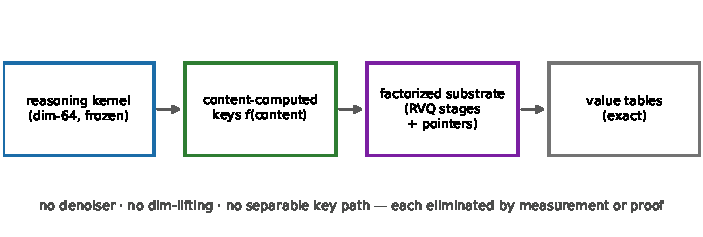
\includegraphics[width=0.92\linewidth]{figures/F3_architecture}
\caption{The surviving architecture. Each absence beneath the diagram is an elimination from
Table~\ref{tab:elim}, not a design preference.}
\label{fig:arch}
\end{figure}

\begin{figure}[t]\centering
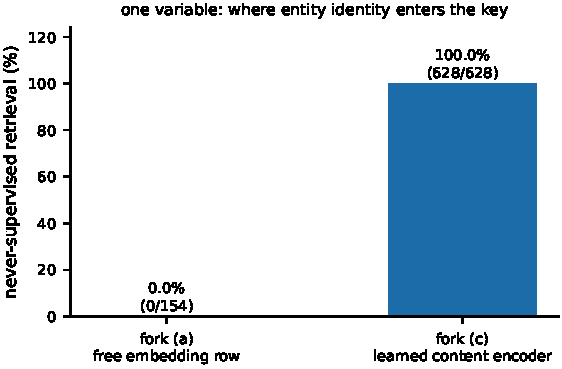
\includegraphics[width=0.55\linewidth]{figures/F2_fork}
\caption{The fork (a)/(c) exhibit: one variable, same evaluator, same day. Identity entering as a
free embedding row gives \textbf{0.0\%} never-supervised retrieval; identity entering through
content gives \textbf{100.0\%}, under a stricter holdout with less data. \textbf{Never-supervised
only} --- the pooled end-to-end figures are excluded for the reason in \S\ref{sec:fork}. Fork (a)'s
denominator is derived: 191 unseen queries less the 37 whose entity embedding was trained elsewhere
(M2 \S11.3), a derivation the loader re-checks against that count on every build.}
\label{fig:fork}
\end{figure}
